\section{Main Tracking Results}
The strongest positive evidence remains the fixed Controller B tracking experiments. Table~\ref{tab:main} is generated from the independently recomputed historical statistics, without pooling stages. Its provenance file records the raw per-start CSVs and hashes.

\begin{center}\small
\begin{tabular}{lrrr}\toprule
Comparison & Mean & 95\% CI & Wins\\\midrule
4: Dir--Mc & 6.75 & [1.24, 14.58] & 4/5 \\
4: Dir--Base & 10.06 & [5.77, 13.03] & 5/5 \\
5A: Dir--Mc & 8.60 & [4.72, 12.20] & 5/5 \\
5A: Dir--Base & 5.14 & [2.42, 8.16] & 5/5 \\
5B: budget & 2.59 & [2.11, 3.07] & 5/5 \\
\bottomrule\end{tabular}
\refstepcounter{table}\label{tab:main}
\par\smallskip Table \thetable: Paired return differences in units of $10^{-4}$. CIs are within-stage seed bootstrap intervals; no cross-stage pooling.
\end{center}


Direction supervision improves over the matched Base model in all five Stage4 seeds and in all five independent Stage5A confirmation seeds. The Stage5A mean difference is $5.14\times10^{-4}$ in physical return. Against Mc, Stage4 improves in four of five seeds, while Stage5A improves in five of five. The effect sizes and seed variability are more informative than calling all of these comparisons statistically significant.

The Stage5B budget comparison assigns the finite-difference control-step allowance to additional dynamics training data for Base. Dir still improves in five of five seeds, with mean difference $2.59\times10^{-4}$. This rules out one specific extra-data explanation under that protocol; it does not establish equality of wall-clock compute or all possible uses of the simulator budget.

\begin{center}
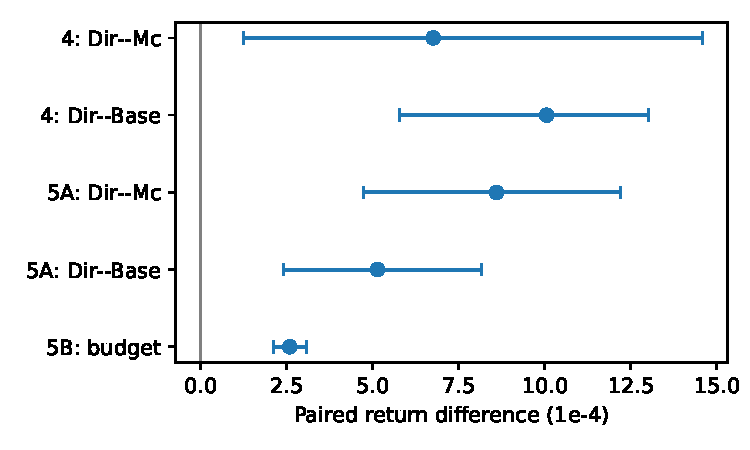
\includegraphics[width=\columnwidth]{figures/historical.pdf}
\end{center}
\noindent\small Figure: Mean paired physical-return differences and seed-bootstrap intervals. Stage4, Stage5A and Stage5B remain separate experiments.\normalsize

Architectural controls provide additional evidence for the command bottleneck: the Stage5C Base comparison improves over the auxiliary-command and observable-memory MLP controls in five of five seeds. These controls should be described through their actual input and parameter budgets, rather than called generic state-of-the-art baselines. The final submission still needs an externally motivated objective baseline such as a matched PAML/GAMPS adaptation.

We restrict the main claim to the evaluated tracking distributions. Later independent controller-randomization seeds support Dir over Base, but comparisons with Mc remain uncertain. Reach does not support the same performance claim. Neither diagnostic oracle outcomes nor multiple starts from the same checkpoint enlarge the sample size of this main table.
